
	\subsection{Variational Monte Carlo calculations of the helium atom}
		As a first attempt to solve the ground state energy for the helium
		atom we perform Variational Monte Carlo calculation with a brute force
		Metropolis sampling. We do this with two trial wave functions
		\[
		\psi_{T}({\bf r_{1}},{\bf r_{2}},{\bf r_{12}})=\exp{\left(-\alpha(r_{1}+r_{2})\right)}\exp{\left(\frac{r_{12}}{2(1+\beta r_{12})}\right)},
		\]
		using $\alpha$ and $\beta$ as variational parameters. 
		We run the Variational Monte Carlo calculation over
		different values for the two variables $\alpha$ and $\beta$, 
		with $2\times10^{7}$ cycles in the Monte Carlo simulation, we get the results
		presented in figure \ref{fig:HeliumAlphaBeta}.
		We find the optimal values to be  $\alpha=1.8$ and $\beta=0.94$ CHECK THIS, as we can see in the figures.
		With these values for $\alpha$ and $\beta$ we get an energy of $-2.8979105$ CHECK THIS.
		The parameter $\alpha$ can be interpreted as a parameter for the
		force pulling the electron to the nucleus.


		


		\begin{figure}
			\centering 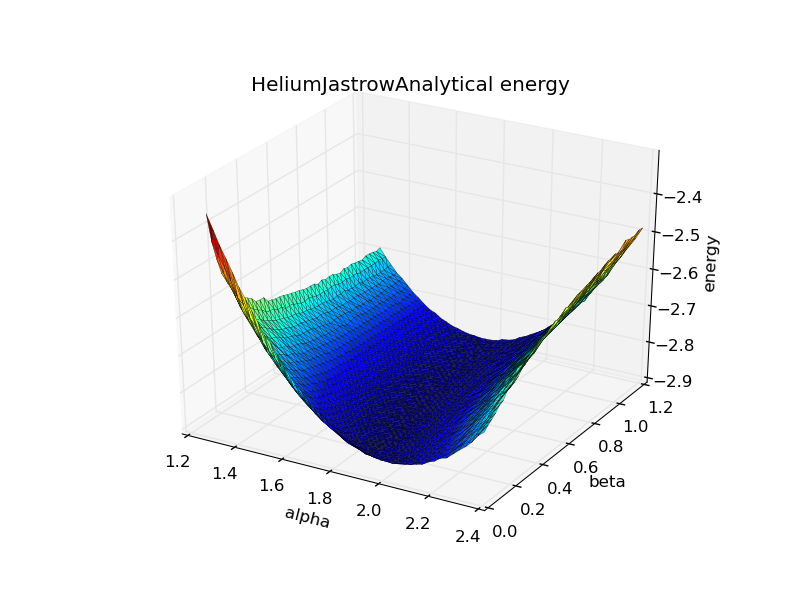
\includegraphics[width=0.49\linewidth]{../figures/HeliumJastrowAnalytical_alpha_beta_energy}
			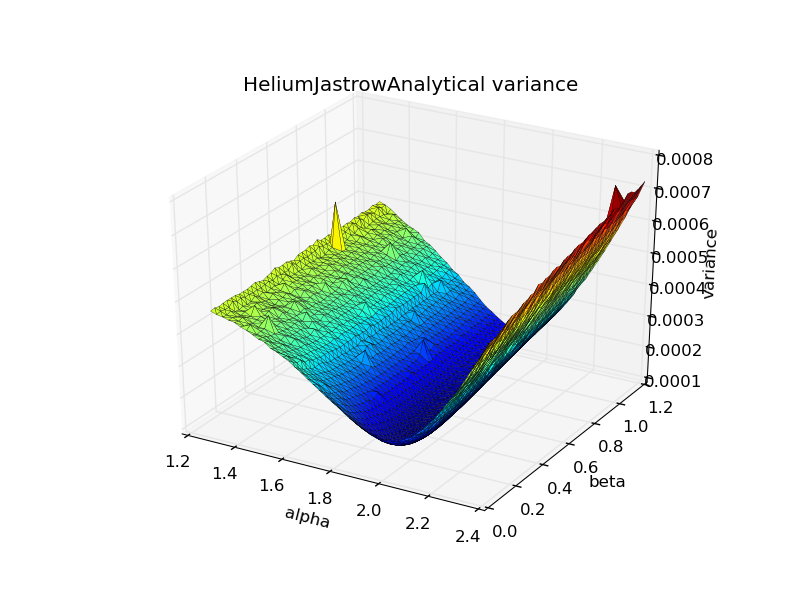
\includegraphics[width=0.49\linewidth]{../figures/HeliumJastrowAnalytical_alpha_beta_variance}
			\protect\caption{Using $\psi_{T}$, plot of the energy versus alpha and beta, and plot of the variance versus $\alpha$ and $\beta$. }
			\label{fig:HeliumAlphaBeta}
		\end{figure}


		\begin{table}
			\centering
			\begin{tabular}{|c|c|c|}
				\hline
				Atom \textbf{UPDATE ME} & VMC & References\tabularnewline
				\hline
				\hline
				Helium $\psi_{T}$ & $-2.8979$ & $-2.9037$ \tabularnewline
				\hline
				Beryllium & $-14.4127$ & $-14.667$\tabularnewline
				\hline
				Neon & $ - $ & $ -128.928 $\tabularnewline
				\hline
			\end{tabular}
			\protect
			\caption{Comparison of energies found with Variational Monte Carlo method and
			energies found in research papers. 	\cite{QUA:QUA560090204}  	\cite{Koput:2011:PCCP}}
			\label{tab:energyReference1}
		\end{table}

		\subsubsection{Alpha and Beta Values}
			\begin{table}
				\center
				\begin{tabular}{| c | c| c |}
				    \hline
				   	\textbf{Trialfunction UPDATE ME} & \(\mathbf{\alpha}\) & \(\mathbf{\beta}\)
				    \\ \hline
				    Helium $\psi_{T}$ & 1.8 & 0.94
				    \\	\hline
				    Beryllium $\psi_{T}$	& 3.8	&	 0.293
				    \\ \hline
				    Neon $\psi_{T}$ & - & -
				    \\	\hline
		  		\end{tabular}
		  		\caption{The values for \(\alpha\) and \( \beta \) where found by doing running Monte Carlo calculation with over a mesh of different \(\alpha\) and \( \beta \) values, with stepssize \(0.02\). Each Monte Carlo run went over \(10 000 	000\), using importance sampling. Then the run with the lowest energy gave the \(\alpha\) and \(\beta\) values.}
			  	\label{tab:alpha_beta1}
			\end{table}

			Table \ref{tab:alpha_beta1} shows the values, for \(\alpha\) and \(\beta\) values, we got from  running several Monte Carlo cycles with different values. As an algorithm to pick out the best values we minimized the energy found in the Monte Carlo runs. The values found are quite uncertain since the variance of the energy was quite high compared to the difference caused by varying the parameters. The variance was more smooth as a function of the parameters, see fig \ref{fig:HeliumAlphaBeta} and should have been used.




		\subsubsection{Computational speed gain by using an analytical local energy}
			By using an analytical expression for the local energy instead of using a numerical derivation in the calculation a speed up of approximately factor \(4\) was achieved, see table \ref{tab:analyticVSNumeric}.

			\begin{table}
				\center
				\begin{tabular}{| c | c | c | c |}
				    \hline
				   	\textbf{Trialfunction UPDATE ME} & Numerical (s) & Analytical (s) & Ratio
				    \\ \hline
				    Helium $\psi_{T}$ & 86.76 & 19.98	& 4.342
				    \\	\hline
				    Beryllium $\psi_{T2}$ & 1918.34  &	 &
					    \\ \hline
				\end{tabular}
				\caption{The time to run a Monte Carlo run with \(10^7\) cycles. The closed expression for the local energy increased the computation time by a significant degree for each trialfunction. }
				\label{tab:analyticVSNumeric}
			\end{table}

		\subsubsection{Calculations using importance sampling}
			We now introduce importance sampling to our calculations. We search for the optimal variables and find them to be $\alpha=FILLME$ and $\beta=FILLME$, which gives an energy of $-FILLME$. The energy and variance as a function of the timestep, $\delta t$ is shown in figure \ref{fig:HeliumTimestep}. BLOCKING. COMPARISON AND COMMENTS. 

			\begin{figure}
				\centering 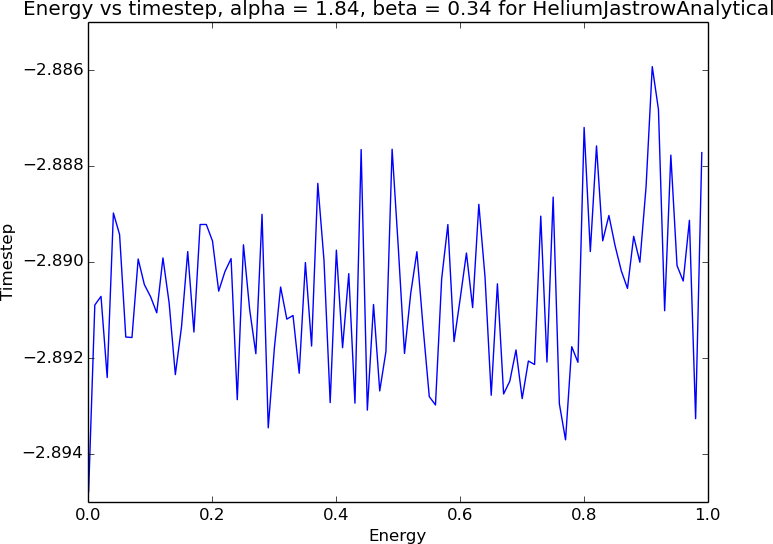
\includegraphics[width=0.45\linewidth]{../figures/HeliumJastrowAnalyticalTimeEnergy}
				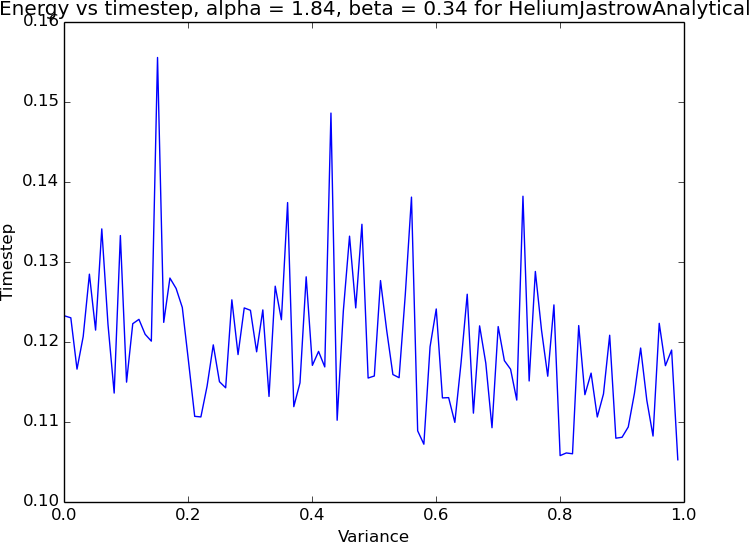
\includegraphics[width=0.45\linewidth]{../figures/HeliumJastrowAnalyticalTimeVariance}
				\protect\caption{Plots for Helium $\psi_{T}$ for the energy versus the timestep, and the variance versus the timestep.}
				\label{fig:HeliumTimestep}
			\end{figure}

		\subsubsection{Onebody density}

		\subsubsection{Conjugate gradient with GTOs}